%!TEX root = ../main.tex

\chapter{Experiments and Results DRAFT\label{chap:experiments_and_results}}

\section{Text representation models}
Table \ref{tab:evaluatinon} presents the evaluation results for the chosen text embedding models.

\subsection{Analysis of results}
\subsubsection{Czech models}
Among the evaluated Czech models, SimCSE-RetroMAE-Small demonstrated the most promising performance.
This model effectively handled both text with diacritics and diacriticless variants, outperforming other models within this category.
Notably, the remaining Czech models achieved performance below the established baseline.

The performance of Czert-B can potentially be attributed to the fact that it was not specifically fine-tuned for the task of generating text embeddings.
This highlights the importance of fine-tuning models for the specific task at hand to optimize their performance.

Regarding the Seznam models, the observed differences in results likely stem from variations in their training processes.
The SimCSE-RetroMAE-Small model emerged as the clear leader within this group, suggesting that the fine-tuning strategy employed with \ac{SimCSE} and \ac{RetroMAE} may be particularly effective for these models.

\subsubsection{Multilingual models}
Among the evaluated multilingual models, all versions of mE5 and LaBSE demonstrated particularly promising performance.
Notably, mE5 achieved the highest overall results within the tested models.
This suggests that the training objectives and architectures employed for these models might be well-suited for capturing semantic similarity across languages, including Czech.
Confusion matrices of \ac{mE5}\textsubscript{Large} evaluation are shown at \reffig{fig:Confusion_matrices}.

Paraphrase-Multilingual-MiniLM-L12-v2 and Paraphrase-Multilingual-MPNet-Base-v2 exhibited strong performance when applied to text containing diacritics.
However, their performance appeared less effective when handling diacriticless text.
This observation suggests that these models might benefit from further training or adaptation specifically tailored for handling variations in Czech text with and without diacritics.

While mBERT and XLM-R did not achieve the same level of success as other models, it's important to acknowledge that the unsupervised training methods they employ (e.g. \ac{MLM} and \ac{NSP}) might not be specifically optimized for the task of assessing semantic similarity.
Alternative training objectives or supervised learning approaches tailored for this task might lead to improved performance from these models in the context of Czech text analysis.

\subsubsection{Monolingual models}

While all monolingual models achieved performance near the established baseline, this is a noteworthy finding considering they were not specifically trained on the Czech language.
This suggests that some level of semantic similarity can be captured between languages with inherent structural similarities, even without targeted training on the target language.
However, it is important to acknowledge that languages possess distinct vocabularies, grammatical structures, and cultural nuances.
Models trained solely on a language like English may struggle to fully grasp the intricacies of Czech text, potentially hindering their ability to achieve optimal performance in tasks involving semantic similarity assessment.

In contrast, several monolingual models, particularly the Nomic Embed models, the small version of GTE, and the large version of GTE-v1.5, exhibited performance exceeding the baseline.
This highlights the potential effectiveness of certain model architectures, even when not specifically trained on the target language.
Further investigation into the specific characteristics of these models that contribute to their success in this context might provide valuable insights for future research.

\begin{figure}[htbp]
    \centering

    \subfloat[Evaluatinon using diacritics tests.]{%
        \centering
        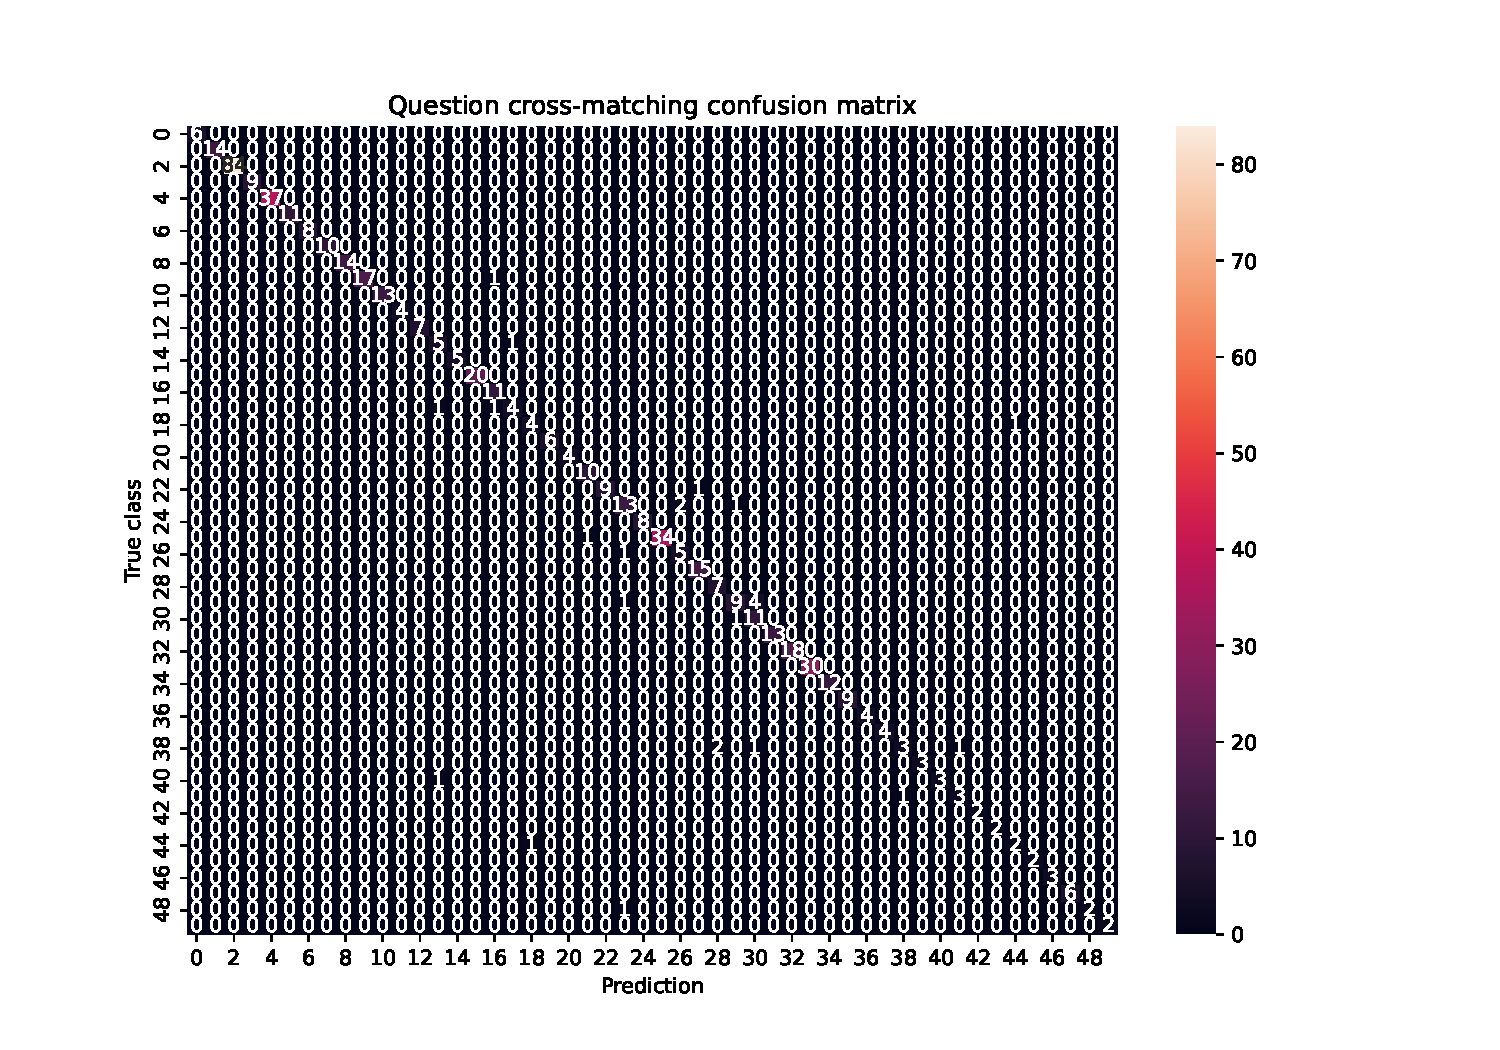
\includegraphics[width=0.54\textwidth,valign=t]{src/fig/pdfs/CM_QMA_FAQ50_diacritics.pdf}
        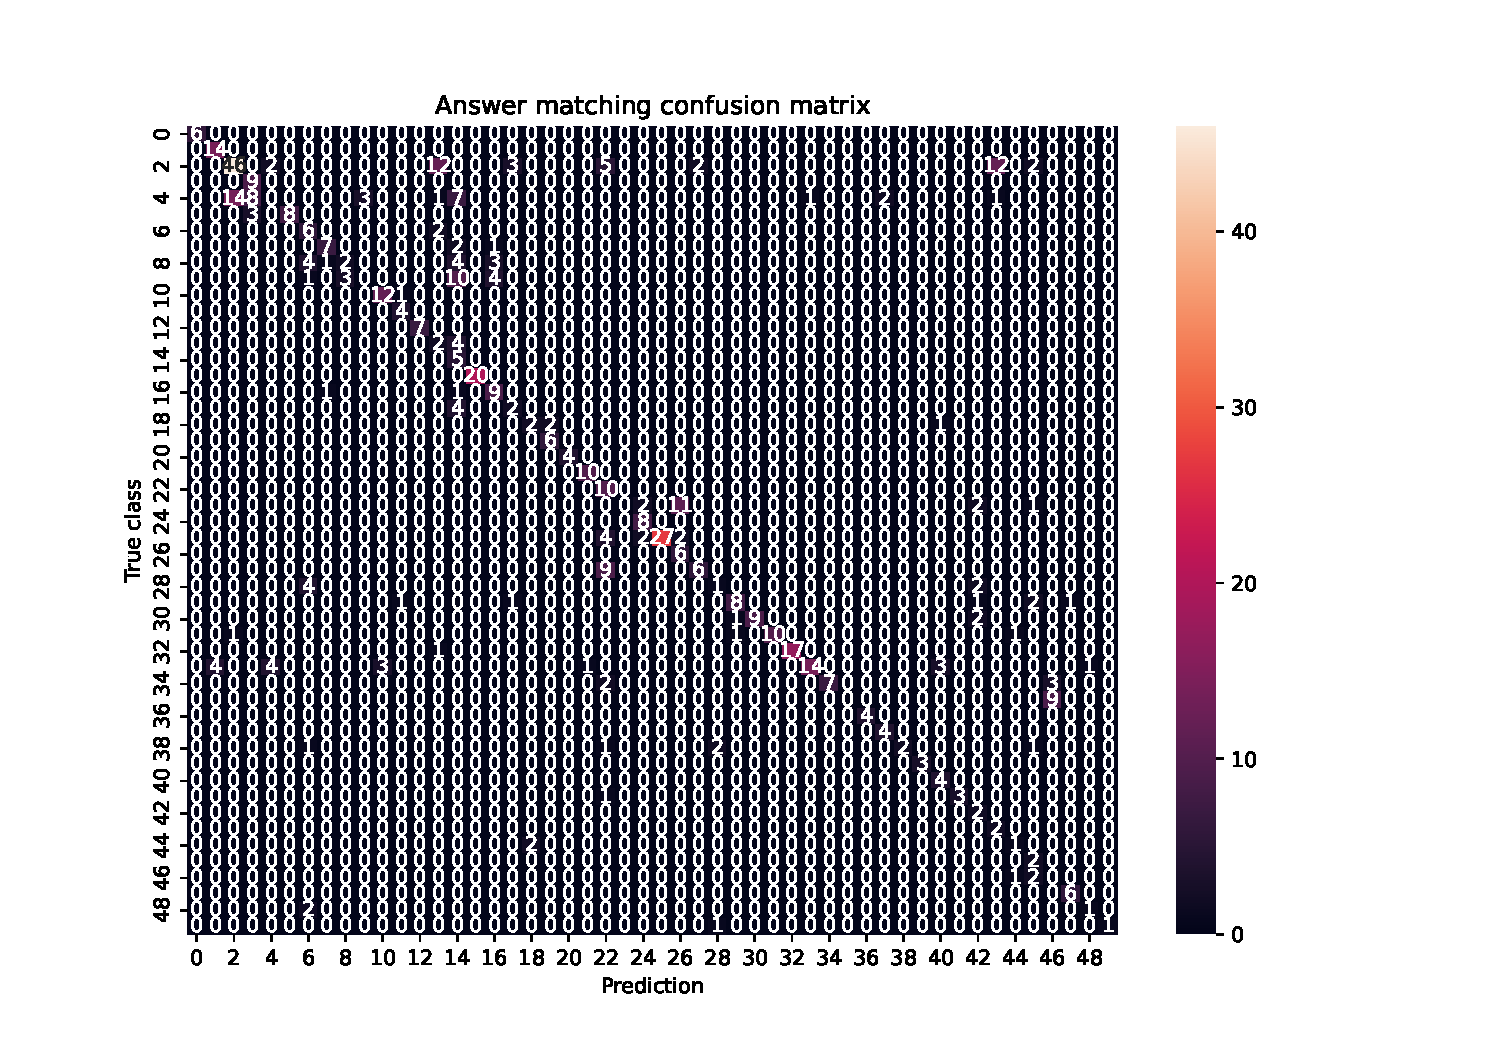
\includegraphics[width=0.54\textwidth,valign=t]{src/fig/pdfs/CM_AMA_FAQ50_diacritics.pdf}
        \label{fig:CM_diacritics}
    }

    \subfloat[Evaluatinon using diacriticless tests.]{%
        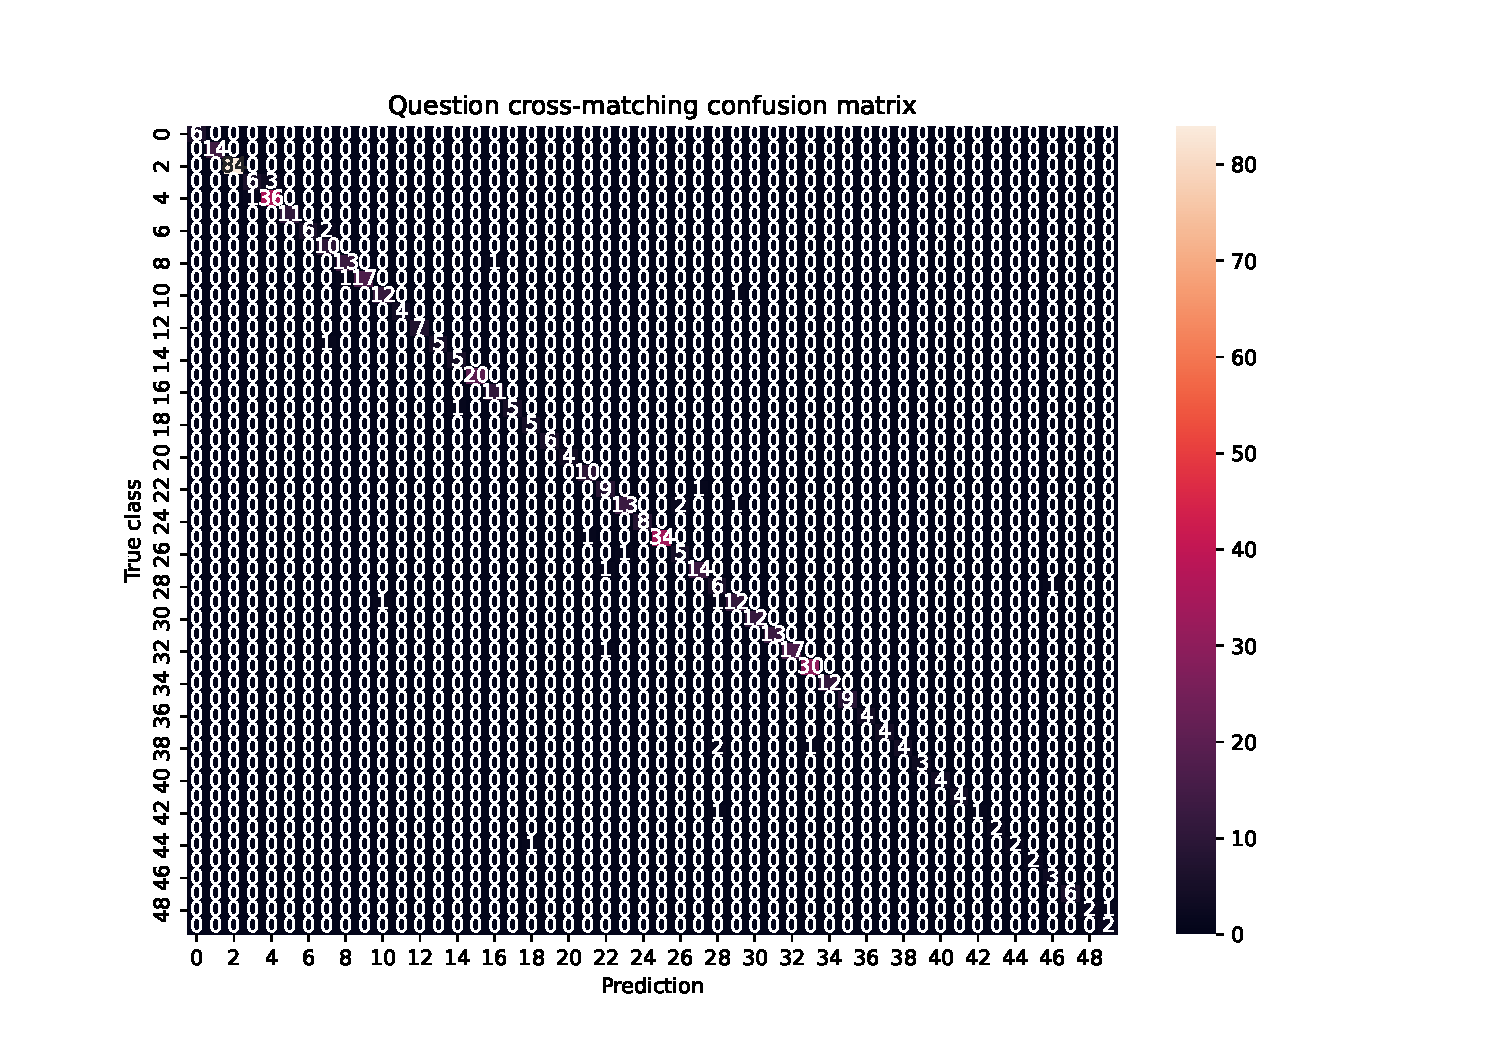
\includegraphics[width=0.54\textwidth,valign=t]{src/fig/pdfs/CM_QMA_FAQ50_diacriticless.pdf}
        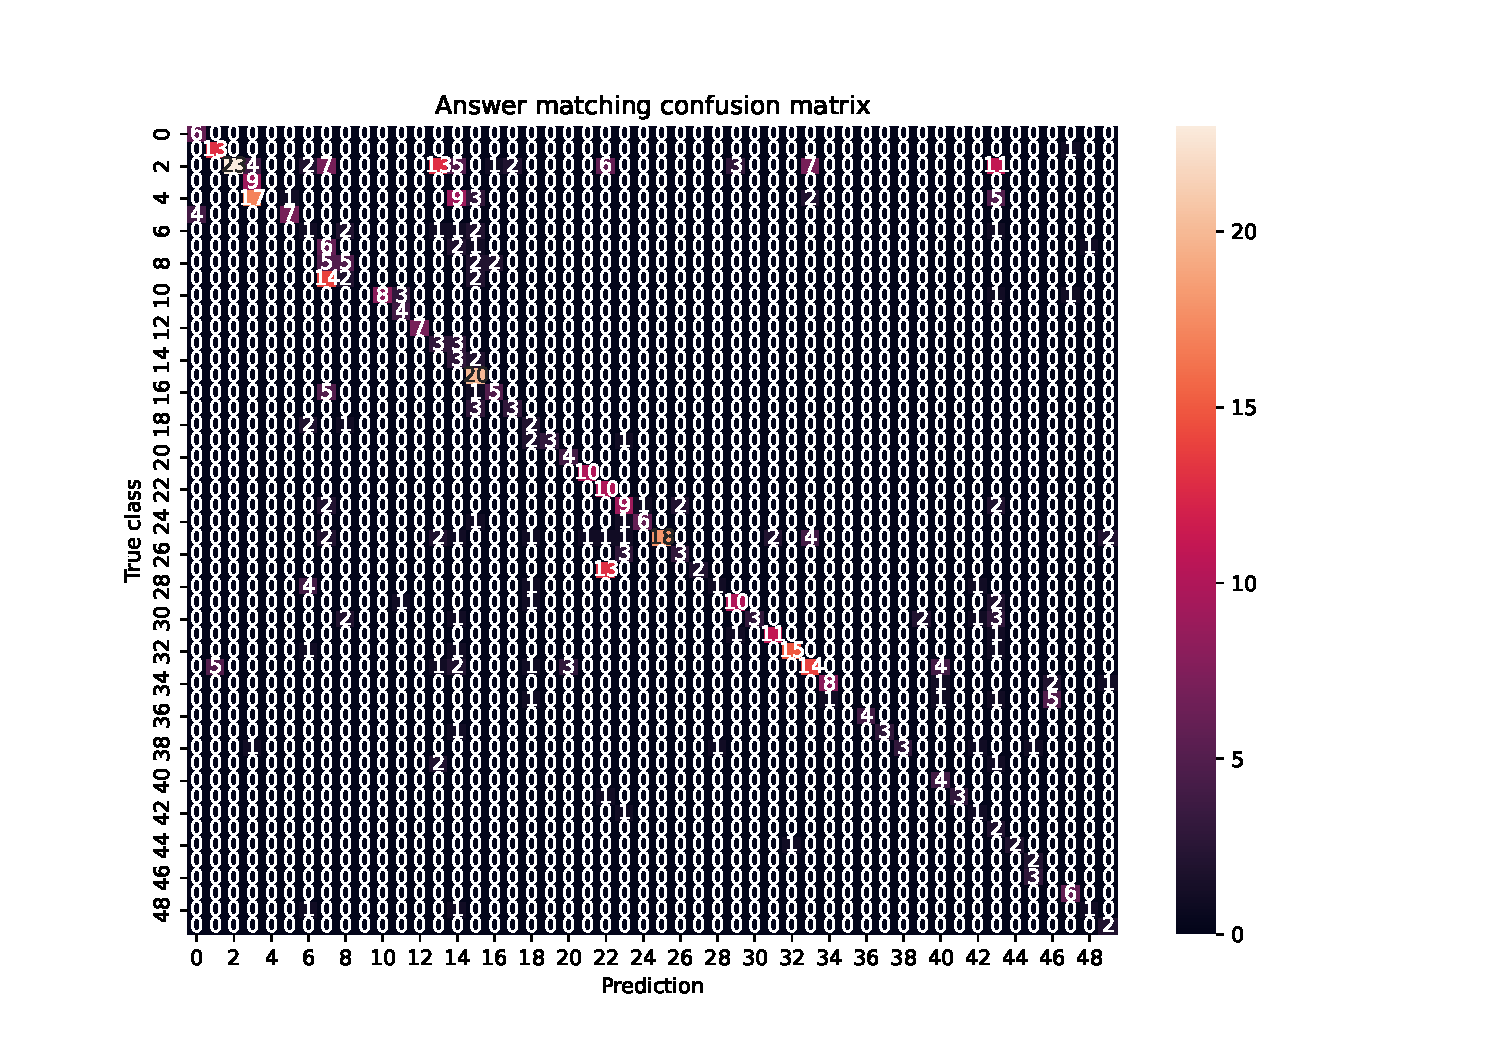
\includegraphics[width=0.54\textwidth,valign=t]{src/fig/pdfs/CM_AMA_FAQ50_diacriticless.pdf}
        \label{fig:CM_diacriticless}
    }

    \caption{Confusion matrices of \ac{mE5}\textsubscript{Large} evaluated using diacritics (a) and diacriticless (b) FAQ50 subsets of UPV FAQ dataset.}
    \label{fig:Confusion_matrices}
\end{figure}

\FloatBarrier

\begin{table*}[ht!]
  \centering
  \begin{tabular}{lcccccc}
    \toprule
    \textbf{Model} & \textbf{QMA}\textsubscript{d} & \textbf{AMA}\textsubscript{d} & \textbf{QMA}\textsubscript{dl} & \textbf{AMA}\textsubscript{dl} & \textbf{\#params} \\
    \hline
    \multicolumn{6}{c}{BASELINE} \\
    \hline
    FastText\textsubscript{diacritics} & 0.8304 & 0.2899 & 0.8110 & 0.2923 & 240M \\
    FastText\textsubscript{diacriticless} & 0.8331 & 0.2864 & 0.8320 & 0.3020 & 229M \\
    \hline
    \multicolumn{6}{c}{CZECH MODELS} \\
    \hline
    Czert-B & 0.8759 & 0.2469 & 0.8388 & 0.0977 & 110M \\
    RetroMAE-Small & 0.8651 & 0.2893 & 0.8634 & 0.2437 & 24M \\
    Dist-MPNet-ParaCrawl & 0.8540 & 0.1089 & 0.8344 & 0.0808 & 24M \\
    Dist-MPNet-CzEng & 0.8705 & 0.0487 & 0.8322 & 0.0426 & 24M \\
    SimCSE-RetroMAE-Small & 0.8682 & 0.3647 & 0.8649 & 0.3316 & 24M \\
    SimCSE-Dist-MPNet-ParaCrawl & 0.8817 & 0.2552 & 0.8602 & 0.2322 & 24M \\
    SimCSE-Dist-MPNet-CzEng & 0.8833 & 0.2278 & 0.8556 & 0.1450 & 24M \\
    SimCSE-Small-E-Czech & 0.8094 & 0.1074 & 0.8160 & 0.0878 & 13M \\
    \hline
    \multicolumn{6}{c}{MULTILINGUAL MODELS} \\
    \hline
    mBERT & 0.8584 & 0.2012 & 0.8361 & 0.1306 & 178M \\
    mE5\textsubscript{Small} & 0.8952 & 0.6078 & 0.8564 & 0.4446 & 118M \\
    mE5\textsubscript{Base} & 0.8961 & 0.6019 & 0.8726 & 0.5134 & 278M \\
    mE5\textsubscript{Large} & \textbf{0.9084} & \textbf{0.6559} & \textbf{0.8944} & \textbf{0.5593} & 560M \\
    LaBSE & 0.8875 & 0.3525 & 0.8594 & 0.3264 & 471M \\
    XLM-R\textsubscript{Base} & 0.8011 & 0.0098 & 0.7701 & 0.0198 & 279M \\
    XLM-R\textsubscript{Large} & 0.7884 & 0.0460 & 0.7411 & 0.0298 & 560M \\
    Distiluse-Base-Multilingual-Cased-v2 & 0.8335 & 0.2978 & 0.7784 & 0.2369 & 135M \\
    Paraphrase-Multilingual-MiniLM-L12-v2 & 0.8502 & 0.4062 & 0.8029 & 0.2576 & 118M \\
    Paraphrase-Multilingual-MPNet-Base-v2 & 0.8752 & 0.4538 & 0.8354 & 0.3174 & 278M \\
    \hline
    \multicolumn{6}{c}{MONOLINGUAL MODELS} \\
    \hline
    UAE-Large-V1 & 0.8241 & 0.2913 & 0.8237 & 0.2931 & 335M \\
    Mxbai-Embed-Large-v1 & 0.8308 & 0.2998 & 0.8302 & 0.2994 & 335M \\
    Mxbai-Embed-2D-Large-v1 & 0.8260 & 0.2511 & 0.8260 & 0.2516 & 335M \\
    Nomic-Embed-v1 & 0.8523 & 0.3553 & 0.8541 & 0.3751 & 137M \\
    Nomic-Embed-v1.5 & 0.8513 & 0.3537 & 0.8520 & 0.3533 & 137M \\
    Ember-v1 & 0.8259 & 0.2971 & 0.8253 & 0.2966 & 335 \\
    GTE\textsubscript{Small} & 0.8549 & 0.3632 & 0.8543 & 0.3634 & 33M \\
    GTE\textsubscript{Base} & 0.8443 & 0.3645 & 0.8437 & 0.3643 & 109M \\
    GTE\textsubscript{Large} & 0.8376 & 0.3345 & 0.8370 & 0.3352 & 335M \\
    GTE-v1.5\textsubscript{Base} & 0.8501 & 0.3336 & 0.8499 & 0.3305 & 137M \\
    GTE-v1.5\textsubscript{Large} & 0.8592 & 0.3294 & 0.8586 & 0.3289 & 434M \\
    BGE-v1.5\textsubscript{Small} & 0.8479 & 0.3816 & 0.8474 & 0.3798 & 33M \\
    BGE-v1.5\textsubscript{Base} & 0.8368 & 0.3246 & 0.8362 & 0.3240 & 109M \\
    BGE-v1.5\textsubscript{Large} & 0.8244 & 0.2938 & 0.8238 & 0.2955 & 335M \\
    GIST-Embedding-v0\textsubscript{Small} & 0.8498 & 0.2664 & 0.8493 & 0.2653 & 33M \\
    GIST-Embedding-v0\textsubscript{Base} & 0.8307 & 0.3023 & 0.8307 & 0.3023 & 109M \\
    GIST-Embedding-v0\textsubscript{Large} & 0.8219 & 0.2579 & 0.8213 & 0.2588 & 335M \\
    TaylorAI/BGE-micro-v2 & 0.8476 & 0.3616 & 0.8475 & 0.3616 & 17M \\
    TaylorAI/GTE-tiny & 0.8492 & 0.3343 & 0.8488 & 0.3342 & 23M \\
    \bottomrule
  \end{tabular}
  \caption{\textbf{Evaliation of models.}
    We show evaluation results where:
    \textbf{QMA}\textsubscript{d} (\textbf{QMA}\textsubscript{dl}) are Question Match Accuracy for the diacritics (diacriticless) model.
    \textbf{AMA}\textsubscript{d} (\textbf{AMA}\textsubscript{d}) are Question Match Accuracy for the diacritics (diacriticless) model.
    \textbf{\#params} is total number of parameters.}
  \label{tab:evaluatinon}
\end{table*}
  

\FloatBarrier

\subsection{Balanced models}
To ensure the effectiveness of the evaluation process, a selection criterion was applied to the initial set of candidate models.
This criterion focused on Question Matching Accuracy and Answer Matching Accuracy for both diacritic and diacriticless models.
Models that exhibited performance below the established baseline for their respective category (diacritic or diacriticless) were excluded from further evaluation.

Additionally, models with lower performance metrics were removed if a smaller, more efficient model demonstrated comparable or superior accuracy.
This approach ensures that the final selection of models for evaluation represents a balance between effectiveness and efficiency.

\begin{table*}[ht!]
    \centering
    \begin{tabular}{lcccccc}
      \toprule
      \textbf{Model} & \textbf{QMA}\textsubscript{d} & \textbf{AMA}\textsubscript{d} & \textbf{QMA}\textsubscript{dl} & \textbf{AMA}\textsubscript{dl} & \textbf{\#params} \\
      \midrule
      SimCSE-RetroMAE-Small & 0.8682 & 0.3647 & 0.8649 & 0.3316 & 24M \\
      GTE\textsubscript{Small} & 0.8549 & 0.3632 & 0.8543 & 0.3634 & 33M \\
      mE5\textsubscript{Small} & 0.8952 & 0.6078 & 0.8564 & 0.4446 & 118M \\
      mE5\textsubscript{Base} & 0.8961 & 0.6019 & 0.8726 & 0.5134 & 278M \\
      mE5\textsubscript{Large} & \textbf{0.9084} & \textbf{0.6559} & \textbf{0.8944} & \textbf{0.5593} & 560M \\

      
      \bottomrule
    \end{tabular}
    \caption{\textbf{Balanced models.}
    We show most factual models according to their efficiency, where:
    \textbf{QMA}\textsubscript{d} (\textbf{QMA}\textsubscript{dl}) are Question Match Accuracy for the diacritics (diacriticless) model.
    \textbf{AMA}\textsubscript{d} (\textbf{AMA}\textsubscript{d}) are Question Match Accuracy for the diacritics (diacriticless) model.
    \textbf{\#params} is total number of parameters.}
    \label{tab:balanced}
  \end{table*}
  

\section{RAG Optimization}

\begin{table*}[ht!]
    \centering
    \begin{tabular}{lc|ccc}
      \toprule
      $S_{chunk}$ & $K$ & ACC & $t_{encoding}$ \\
      \midrule
      256  & 12 & N/A & 26m 46s \\
      512  & 6  & N/A & 34m 14s \\
      1024 & 3  & N/A & N/A \\
      2048 & 2  & N/A & N/A \\
      4096 & 1  & N/A & N/A \\
      \bottomrule
    \end{tabular}
    \caption{\textbf{RAG evaluation with different parameters.}}
    \label{tab:RAG_evaluation}
  \end{table*}
  

\section{TODO: REMOVE Experiments structure}
\begin{itemize}
    \item Present the results of the evaluation for different text representations using analogy tests and confusion matrices.
    \item Discuss the findings regarding the effectiveness of each representation model for capturing semantic relationships in technical text.
    \item Analyze the results from the RAG evaluation, highlighting the impact of different representations and text chunk sizes on answer generation quality and CPU efficiency.
    \item Identify the representation model that achieves a balance between factuality of answers and computational demands.
\end{itemize}
